\chapter{SUPPLEMENTAL MATERIAL FOR CHAPTER III}

\section{Supplemental Figures}
This section includes the supplemental figures referenced in chapter III. Other supplemental files such as spreadsheets, newick trees, and multiple sequence alignments are included in the chapter 3 sub--directory of the zipped supplemental directory submitted with this dissertation. 

\begin{figure}
\centering
	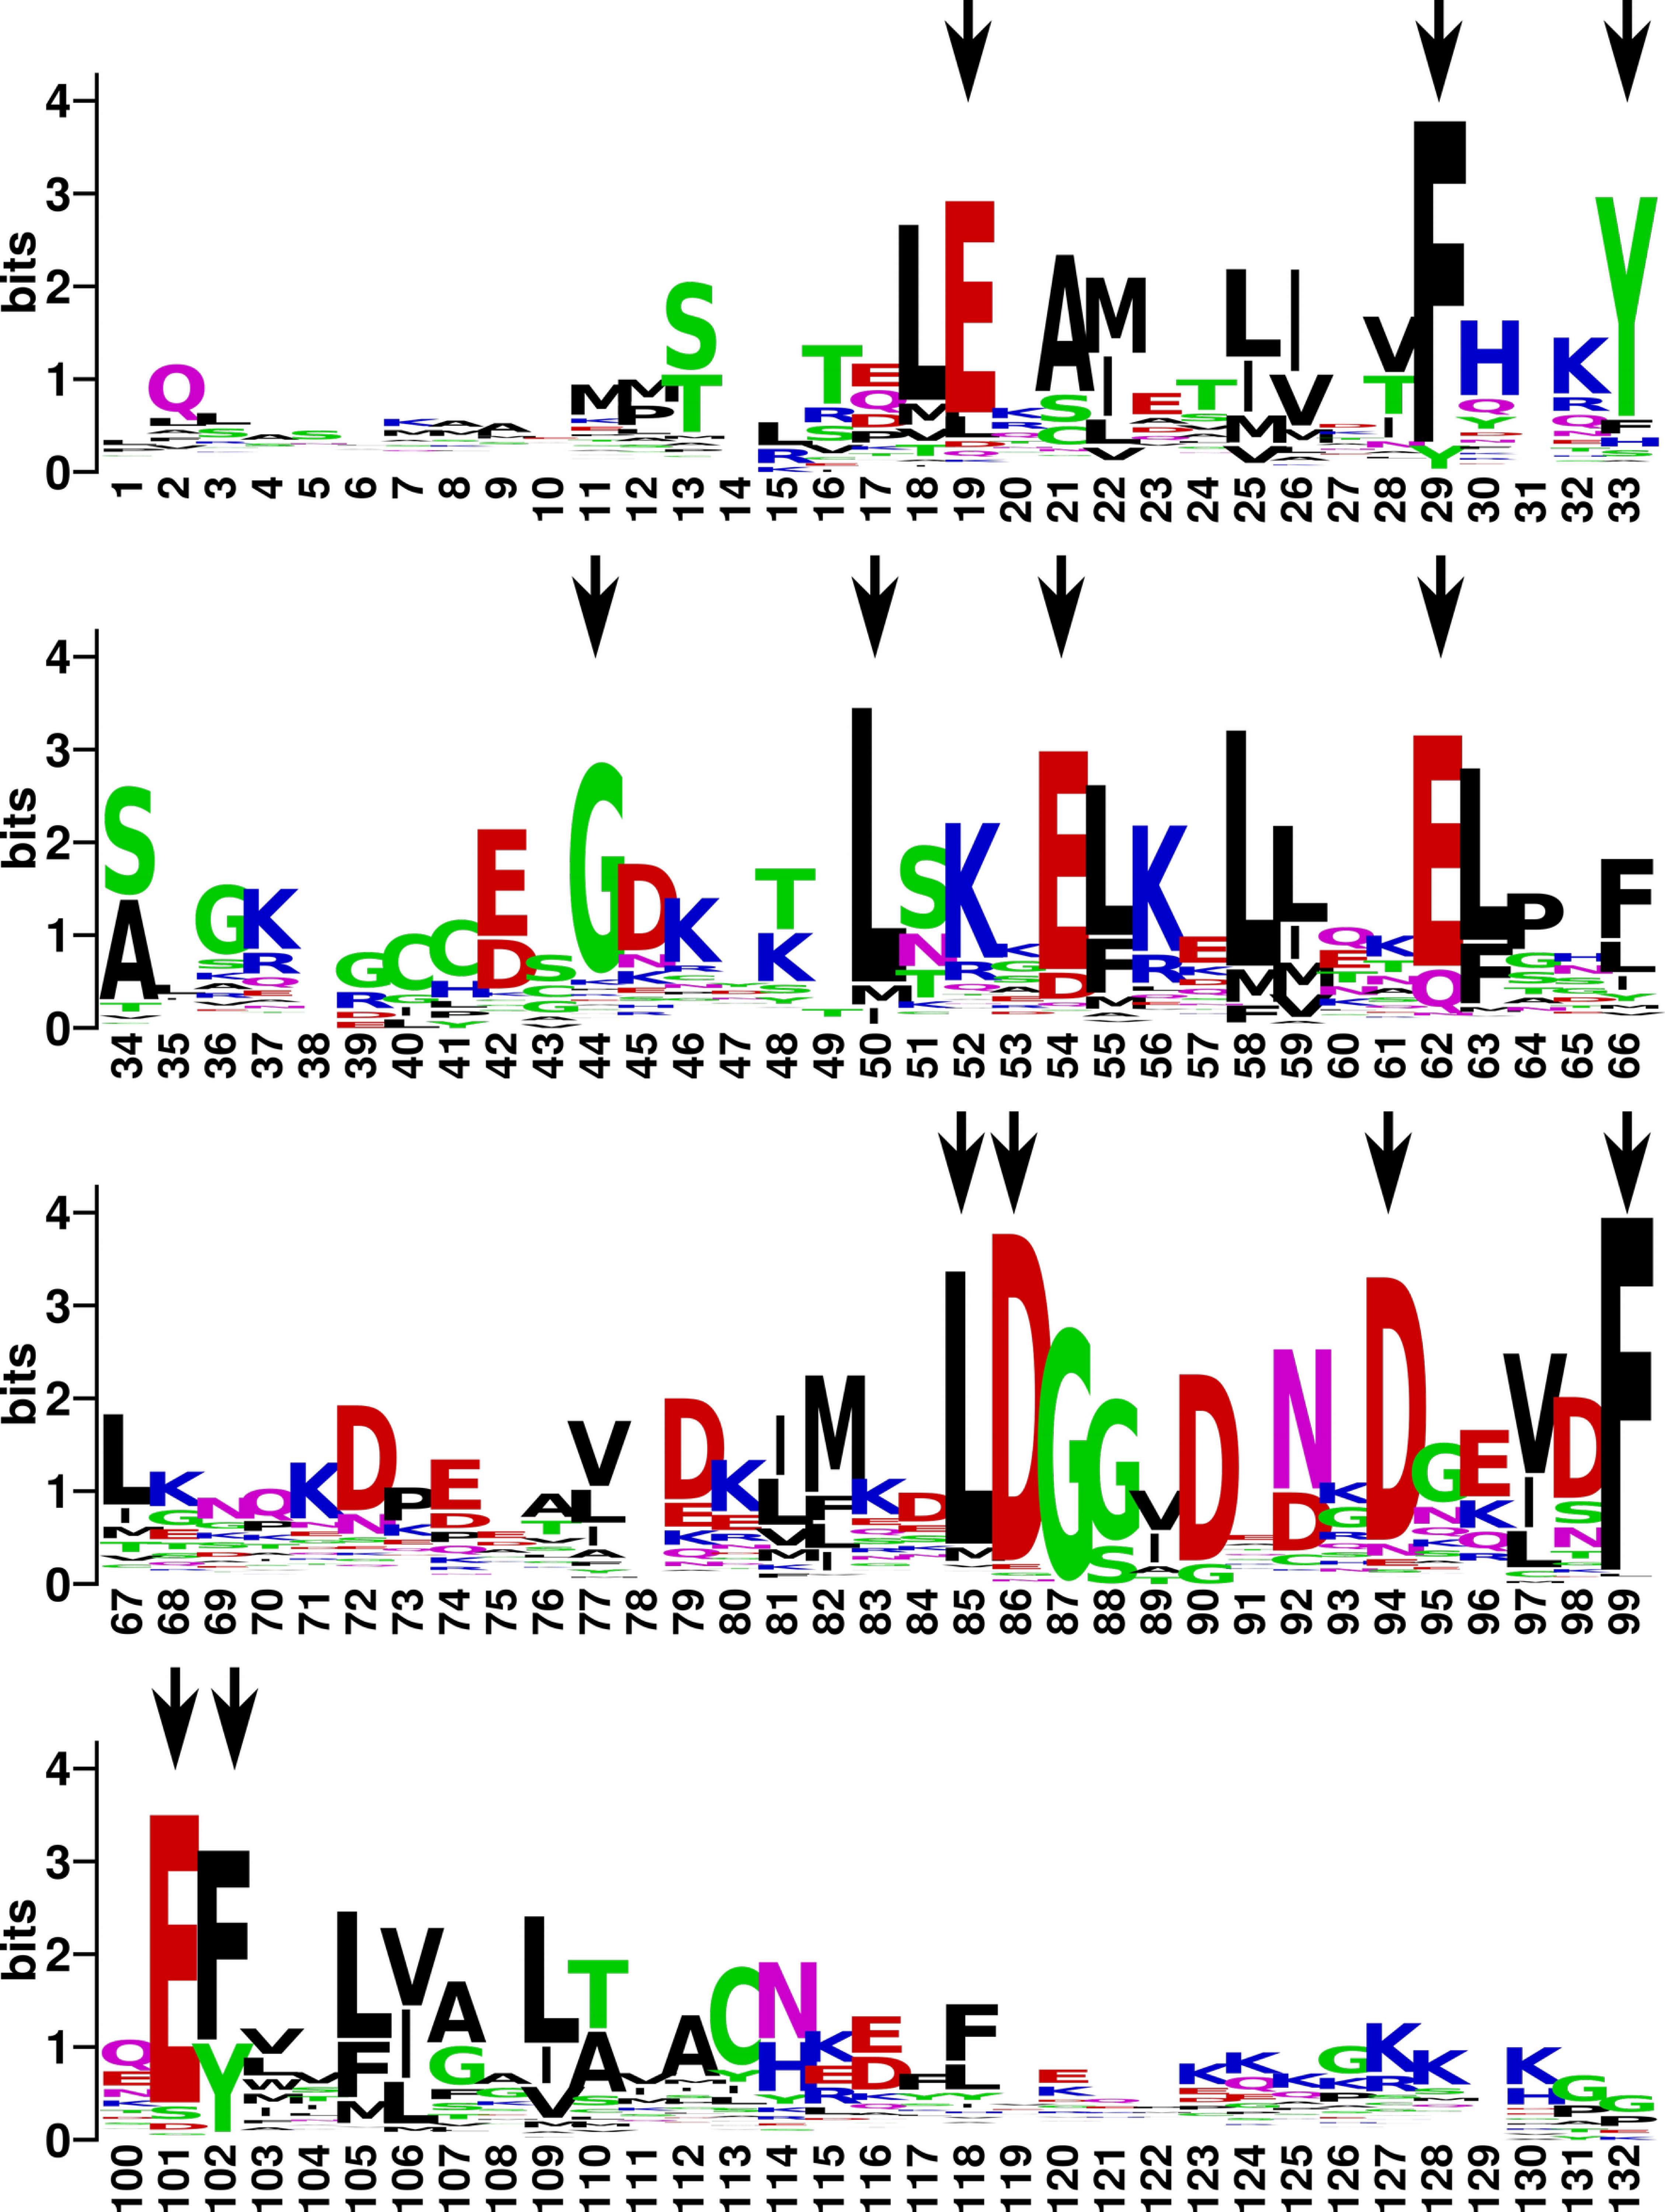
\includegraphics{ch3-FigS1.png} 
\caption[Sequence logos of S100 multiple sequence alignment]{Sequence logo indicates relative frequency of amino acids at each position in the alignment. Taller letters indicate higher frequency at that position. Arrows indicate 13 key residues we used to verify/anchor the alignment.\label{samplefigure}}	
\end{figure}

\begin{figure}
\centering
	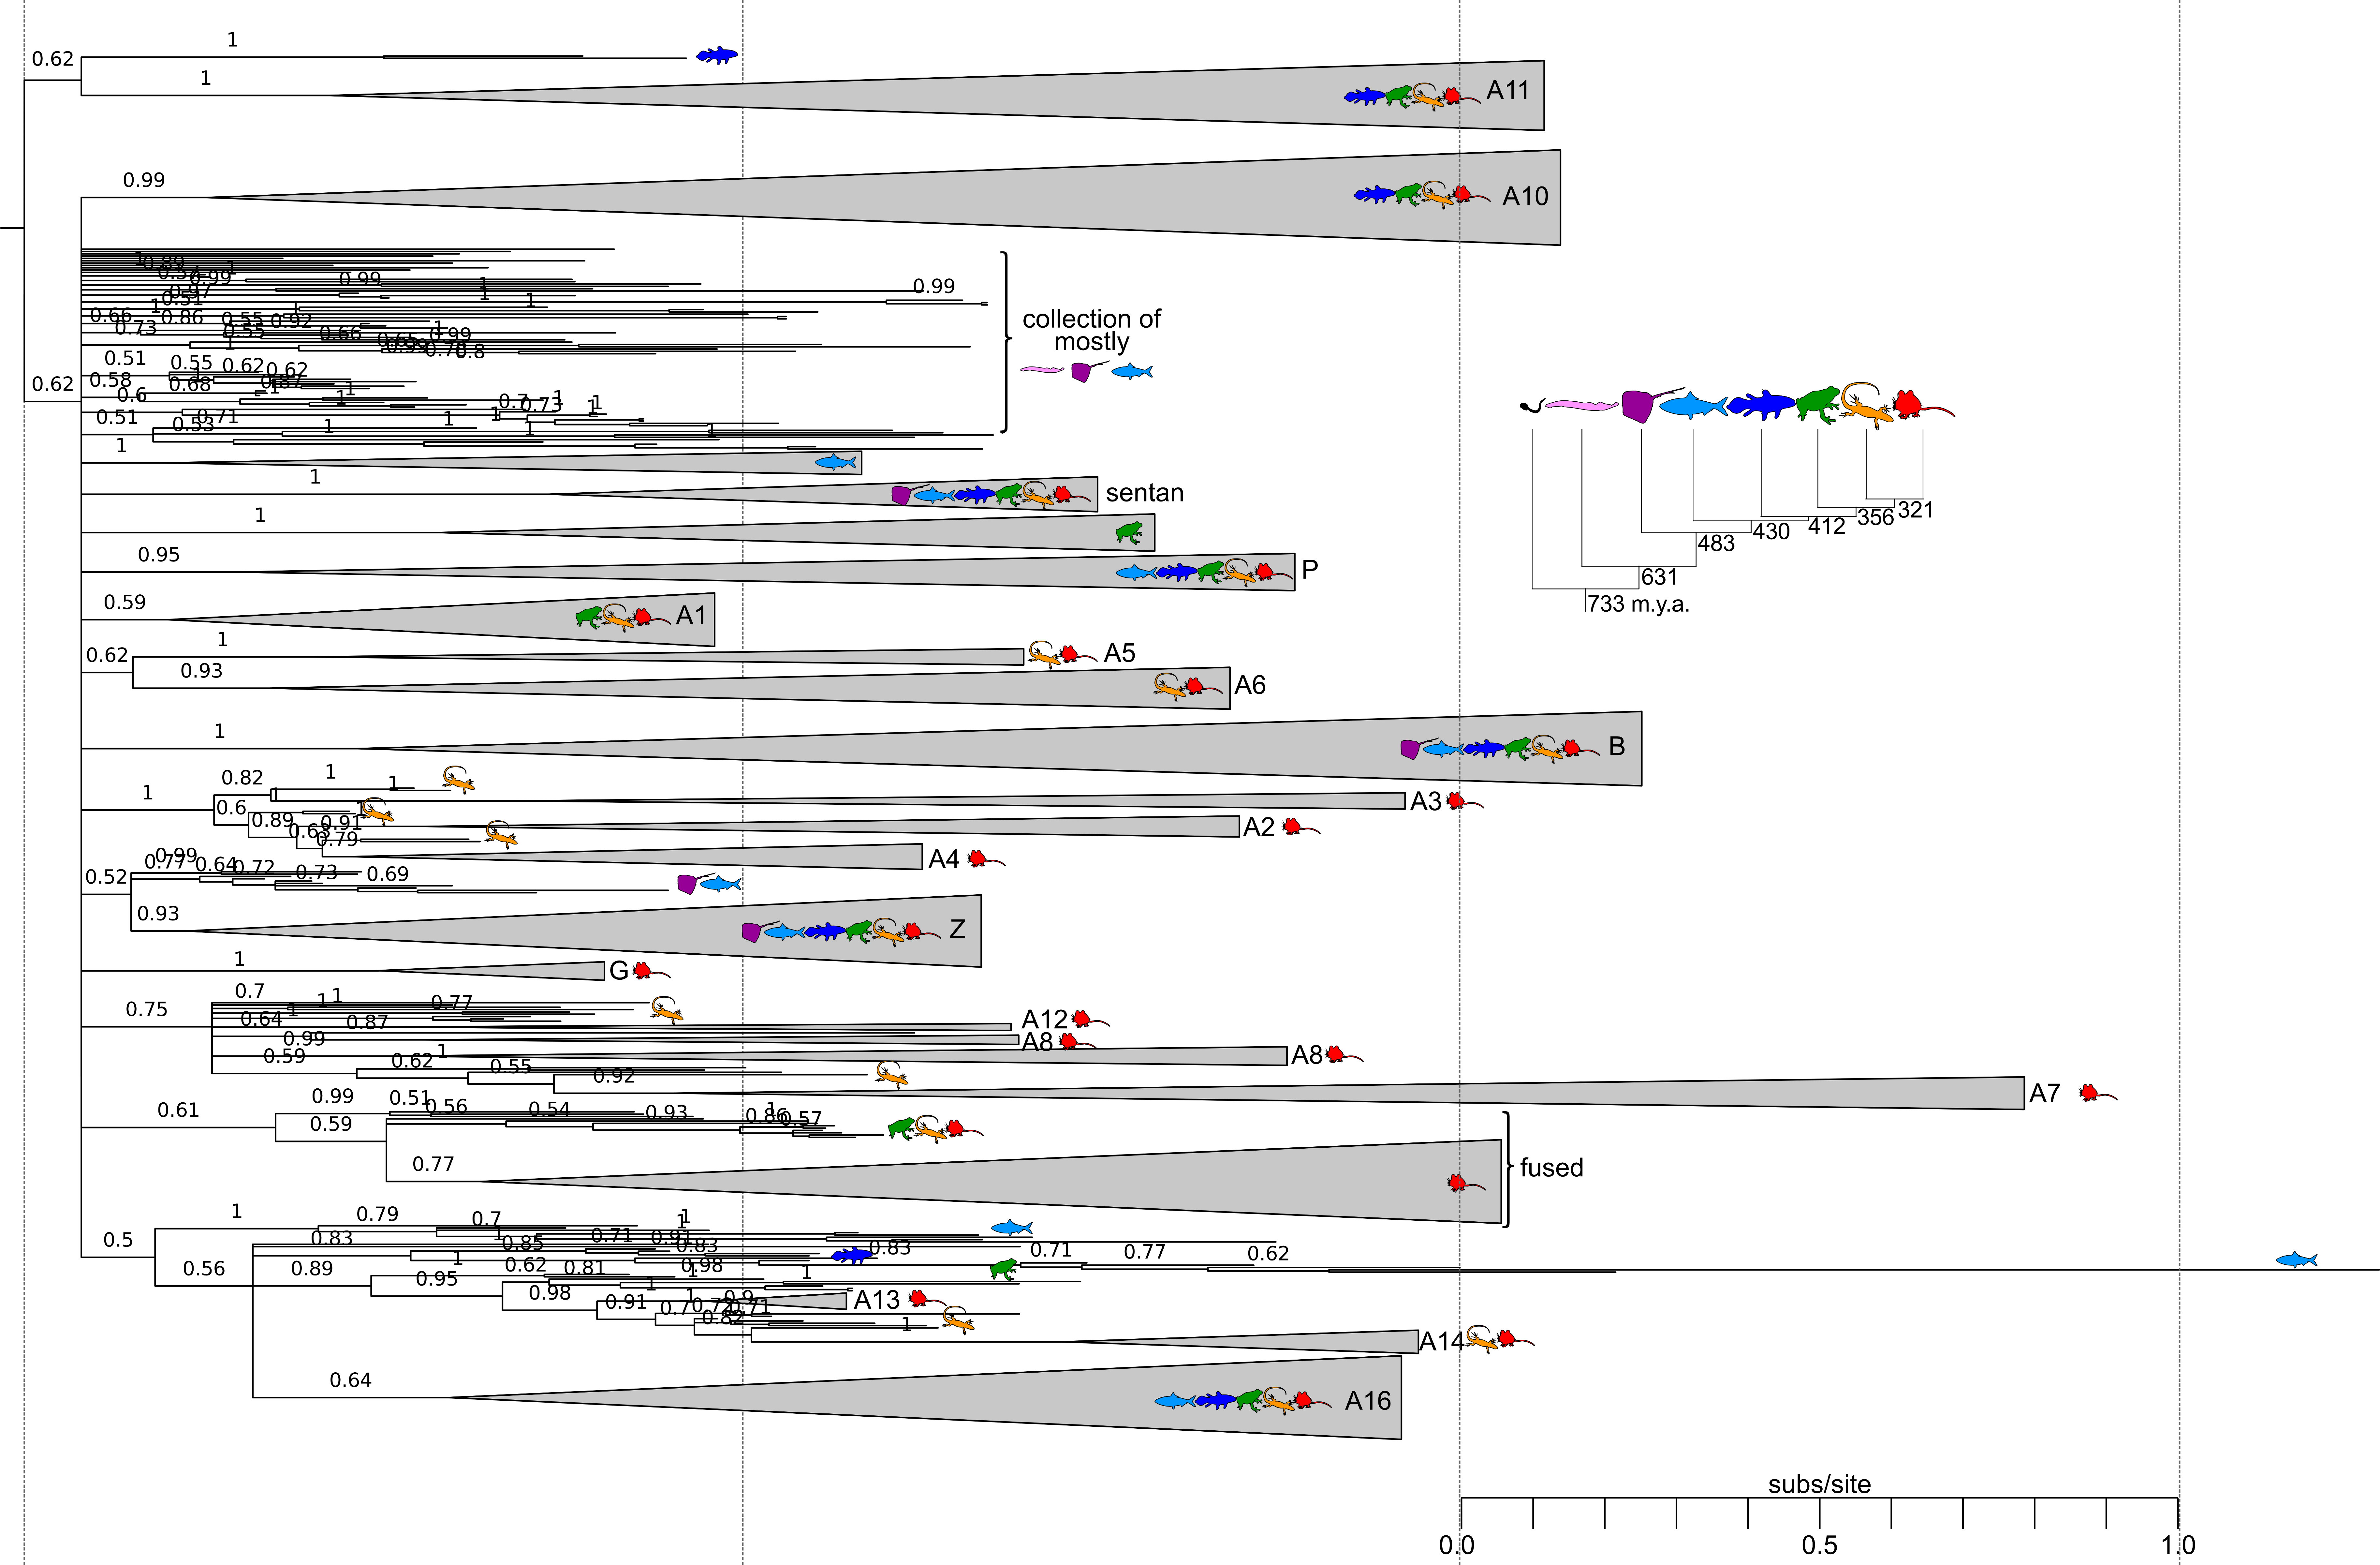
\includegraphics{ch3-S3_fig.png} 
\caption[Bayesian phylogeny of the S100 protein family]{Tree is a majority rule consensus tree, with all nodes with posterior probabilities $<$50\% collapsed into polytomies. Wedges are collapsed clades of shared orthologs, with wedge height denoting number of included taxa and wedge length denoting longest branch length with the clade. Support values are posterior probabilities. Rooting is arbitrary given the poor resolution at the base of the taxonomic tree. Icons indicate taxonomic classes represented within each clade: tunicates (black sea squirt), jawless fishes (pink lamprey), cartilaginous fishes (purple ray), ray-finned fishes (light blue fish), lobe-finned fishes (blue coelacanth), amphibans (green frog), birds/reptiles (yellow lizard), and mammals (red mouse). Inset shows estimated divergence times for each taxonomic class in millions of years before present.\label{samplefigure}}	
\end{figure}


\begin{figure}
\centering
	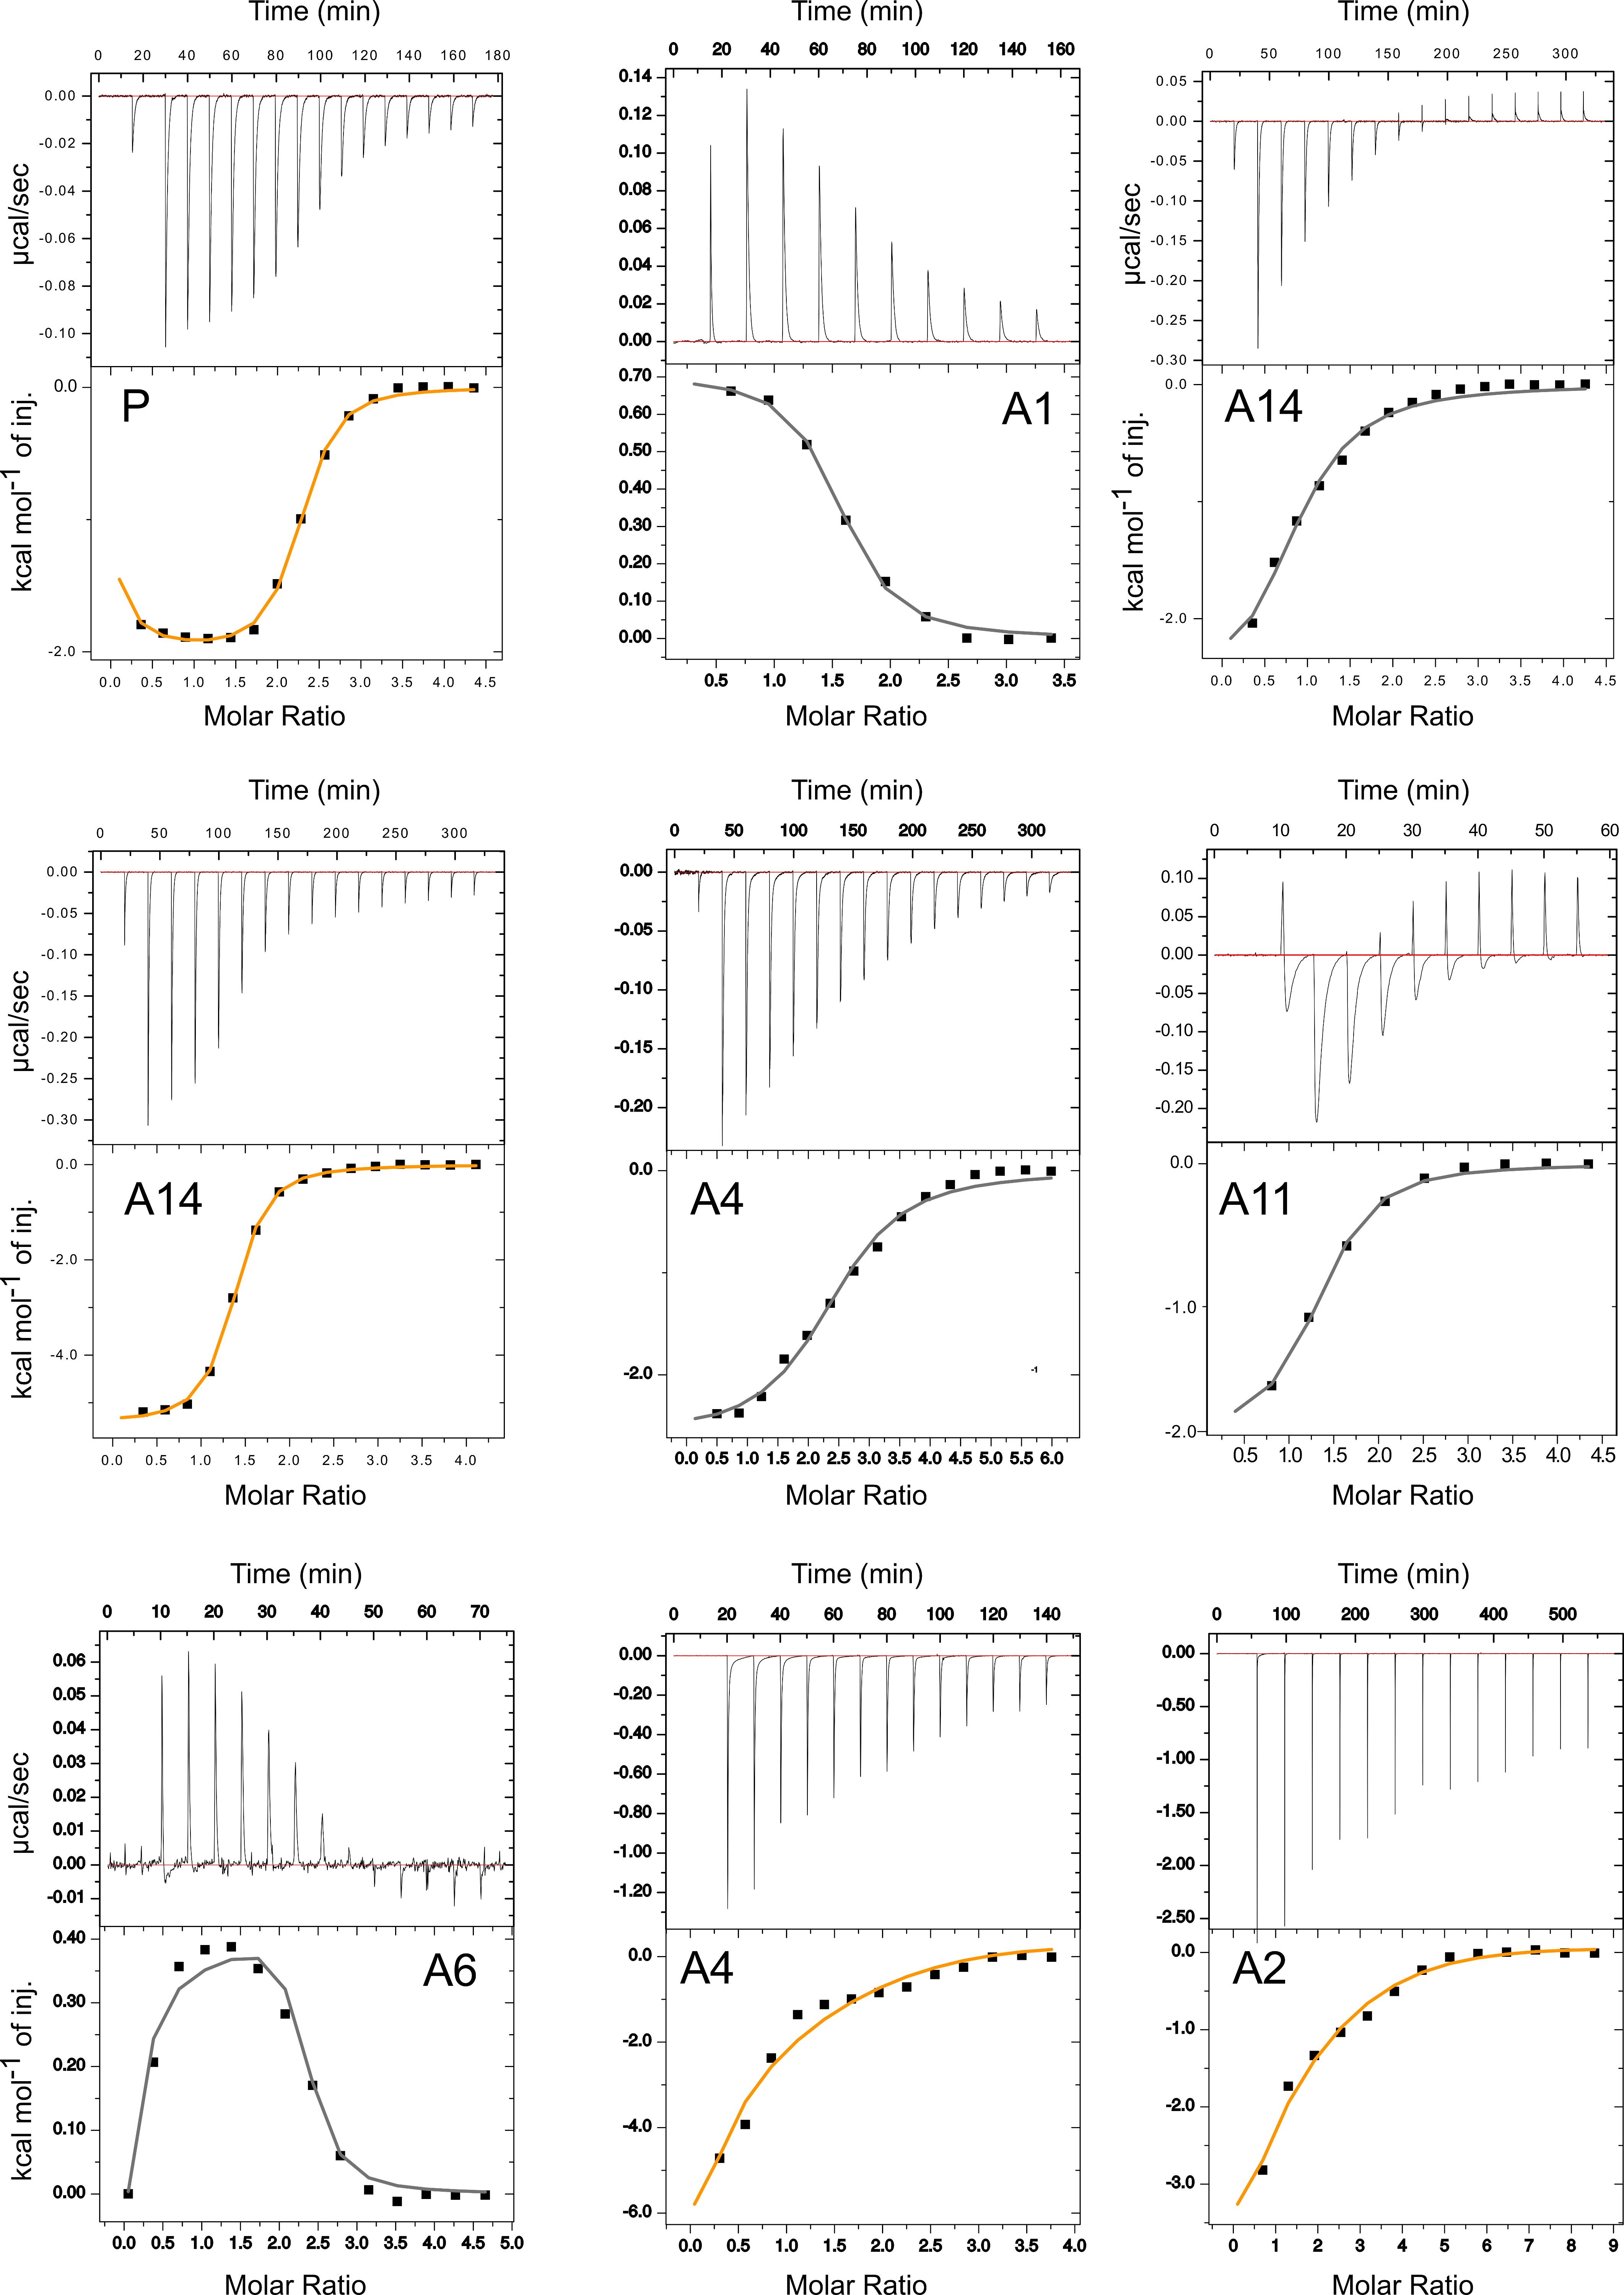
\includegraphics{ch3-S4_fig.png} 
\caption[Representative ITC data and single-site fits]{Each panel is a single human paralog, indicated by the name on the graph. Color of fit indicates metal used as titrant: Zn\textsuperscript{2+} (gray) or Cu\textsuperscript{2+} (copper). Top sub-panel for each panel is a raw power vs. time curve. Bottom sub-panel for each panel is integrated heat versus molar ratio. The model fit is denoted by the heavy line through the fit points.\label{samplefigure}}	
\end{figure}

\begin{figure}
\centering
	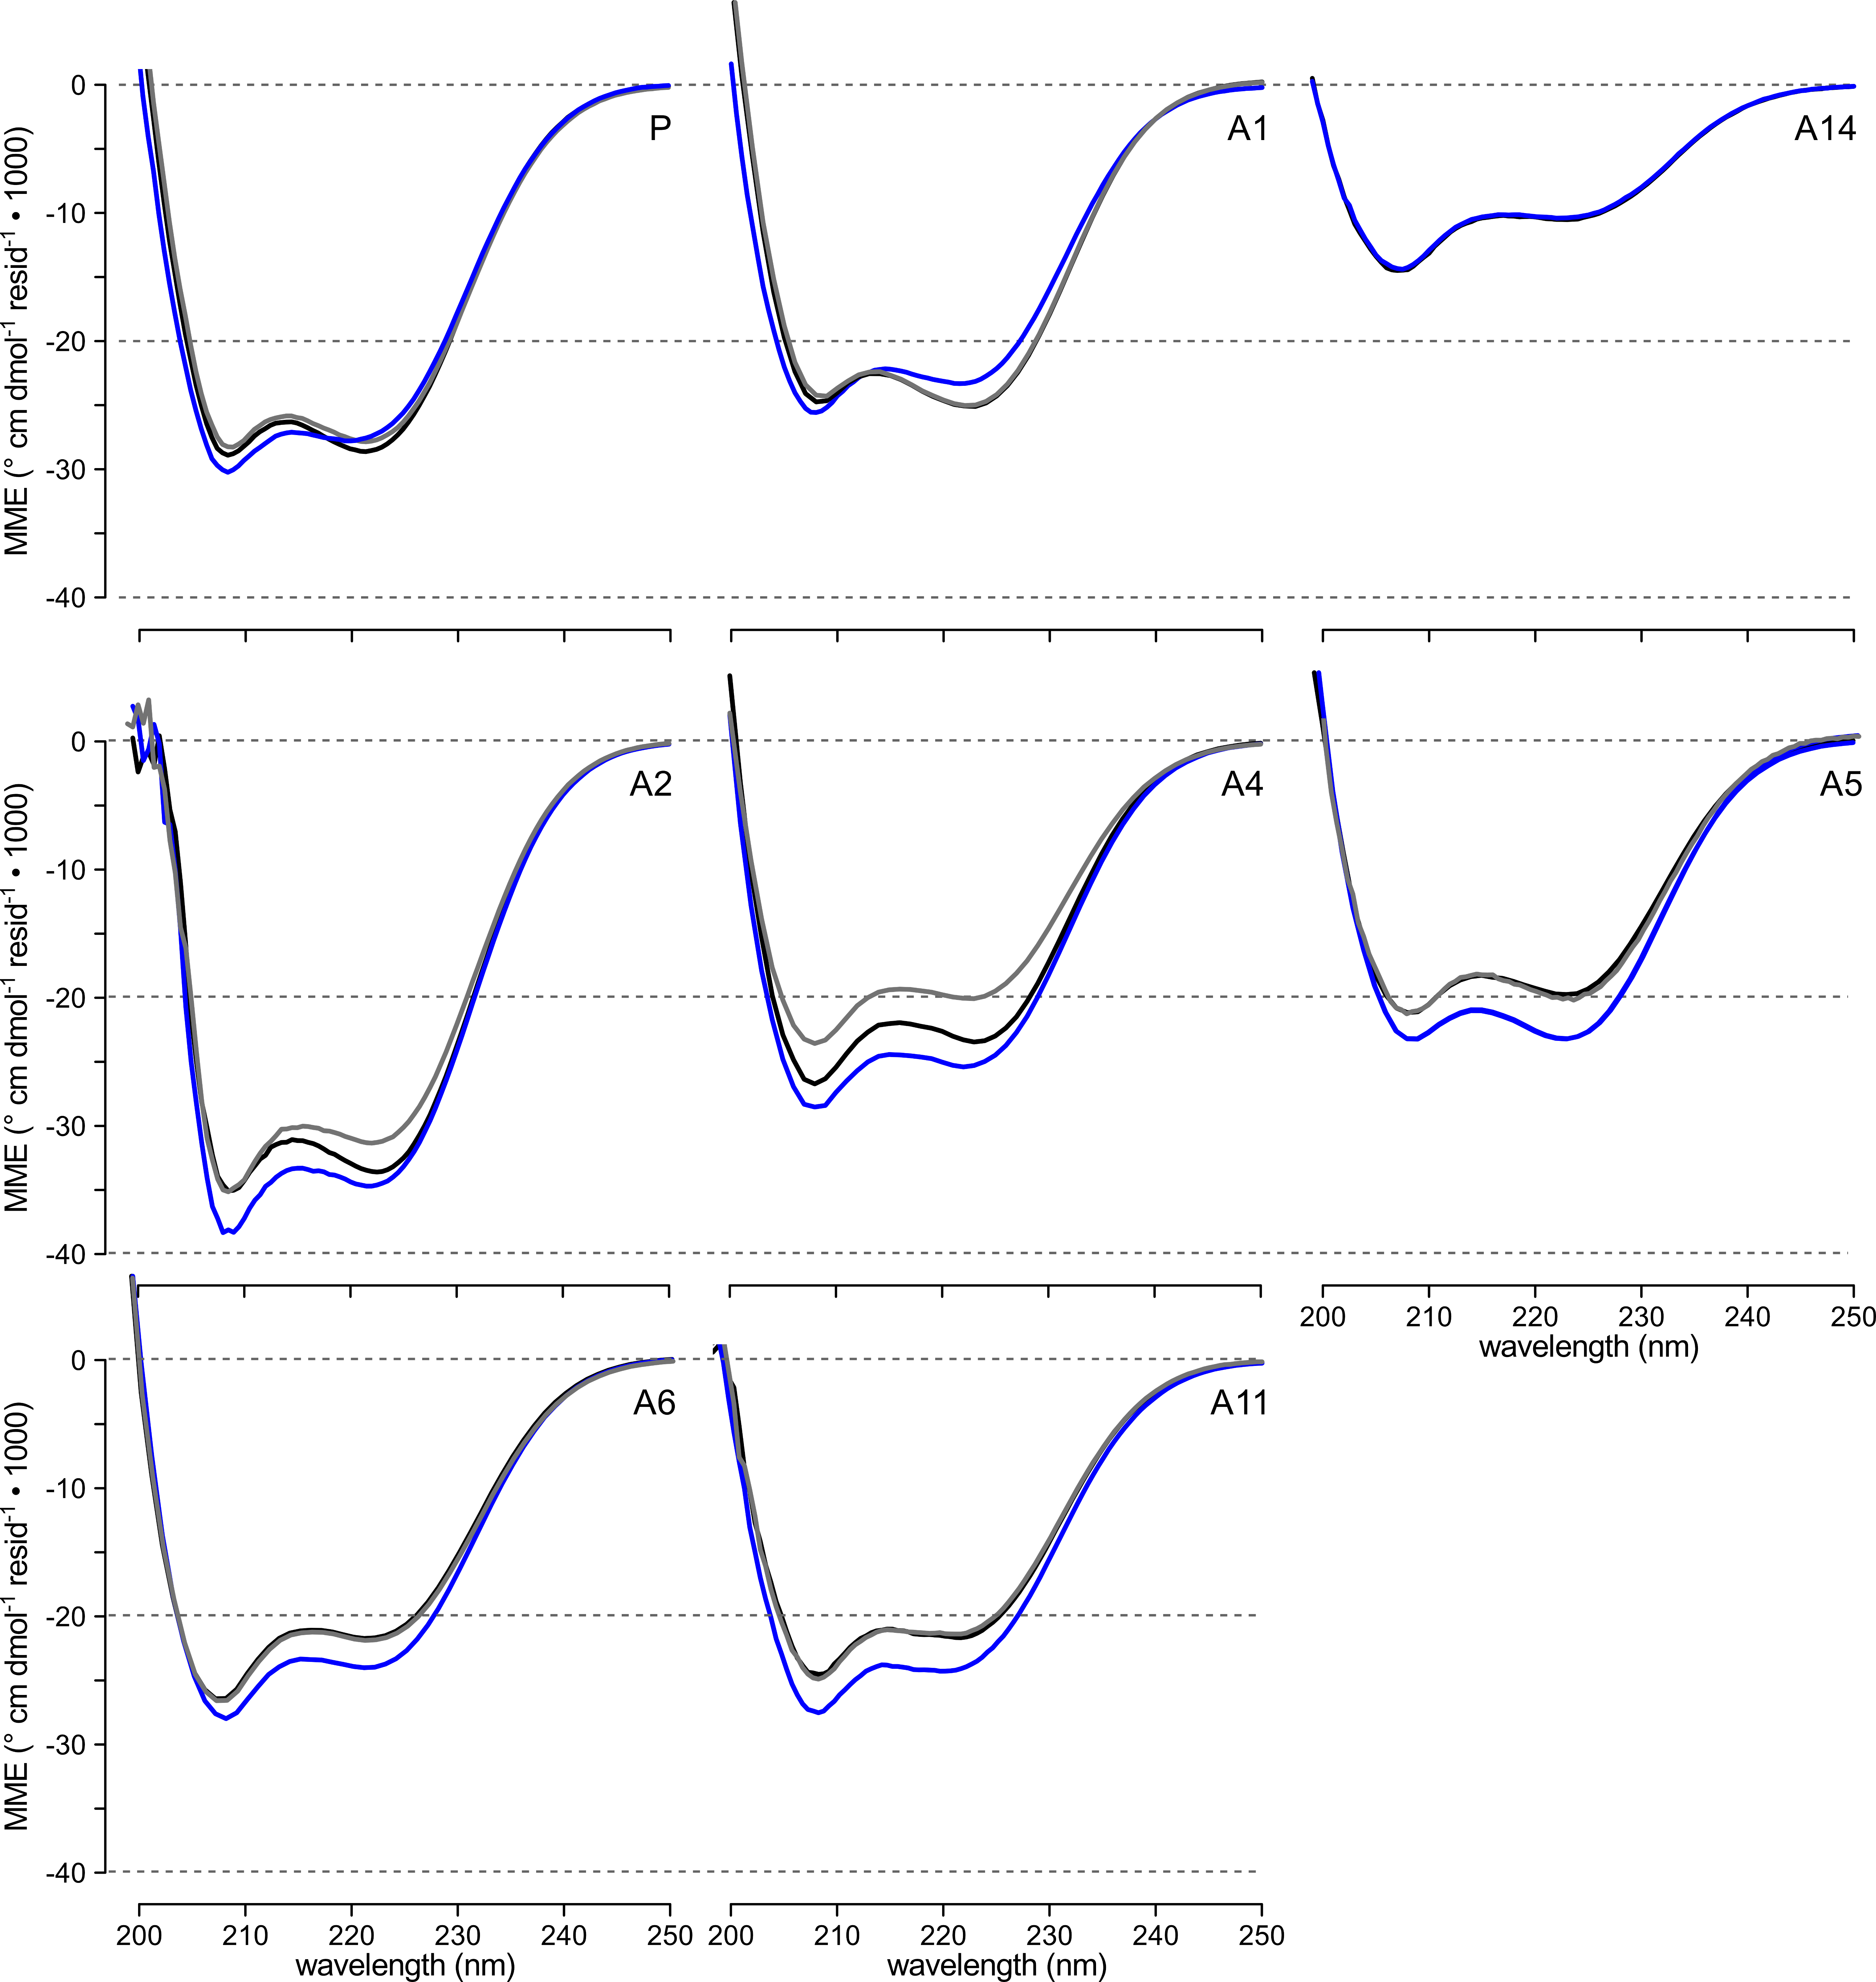
\includegraphics{ch3-S5_fig.png} 
\caption[Far UV CD spectra of S100 proteins]{Curves are far-UV CD spectra (mean molar ellipticity vs. wavelength). Colors represent metal: apo (black), Zn\textsuperscript{2+} (gray), and Ca\textsuperscript{2+} (blue). Paralog is indicated to the right of each spectrum.\label{samplefigure}}	
\end{figure}


\begin{figure}
\centering
	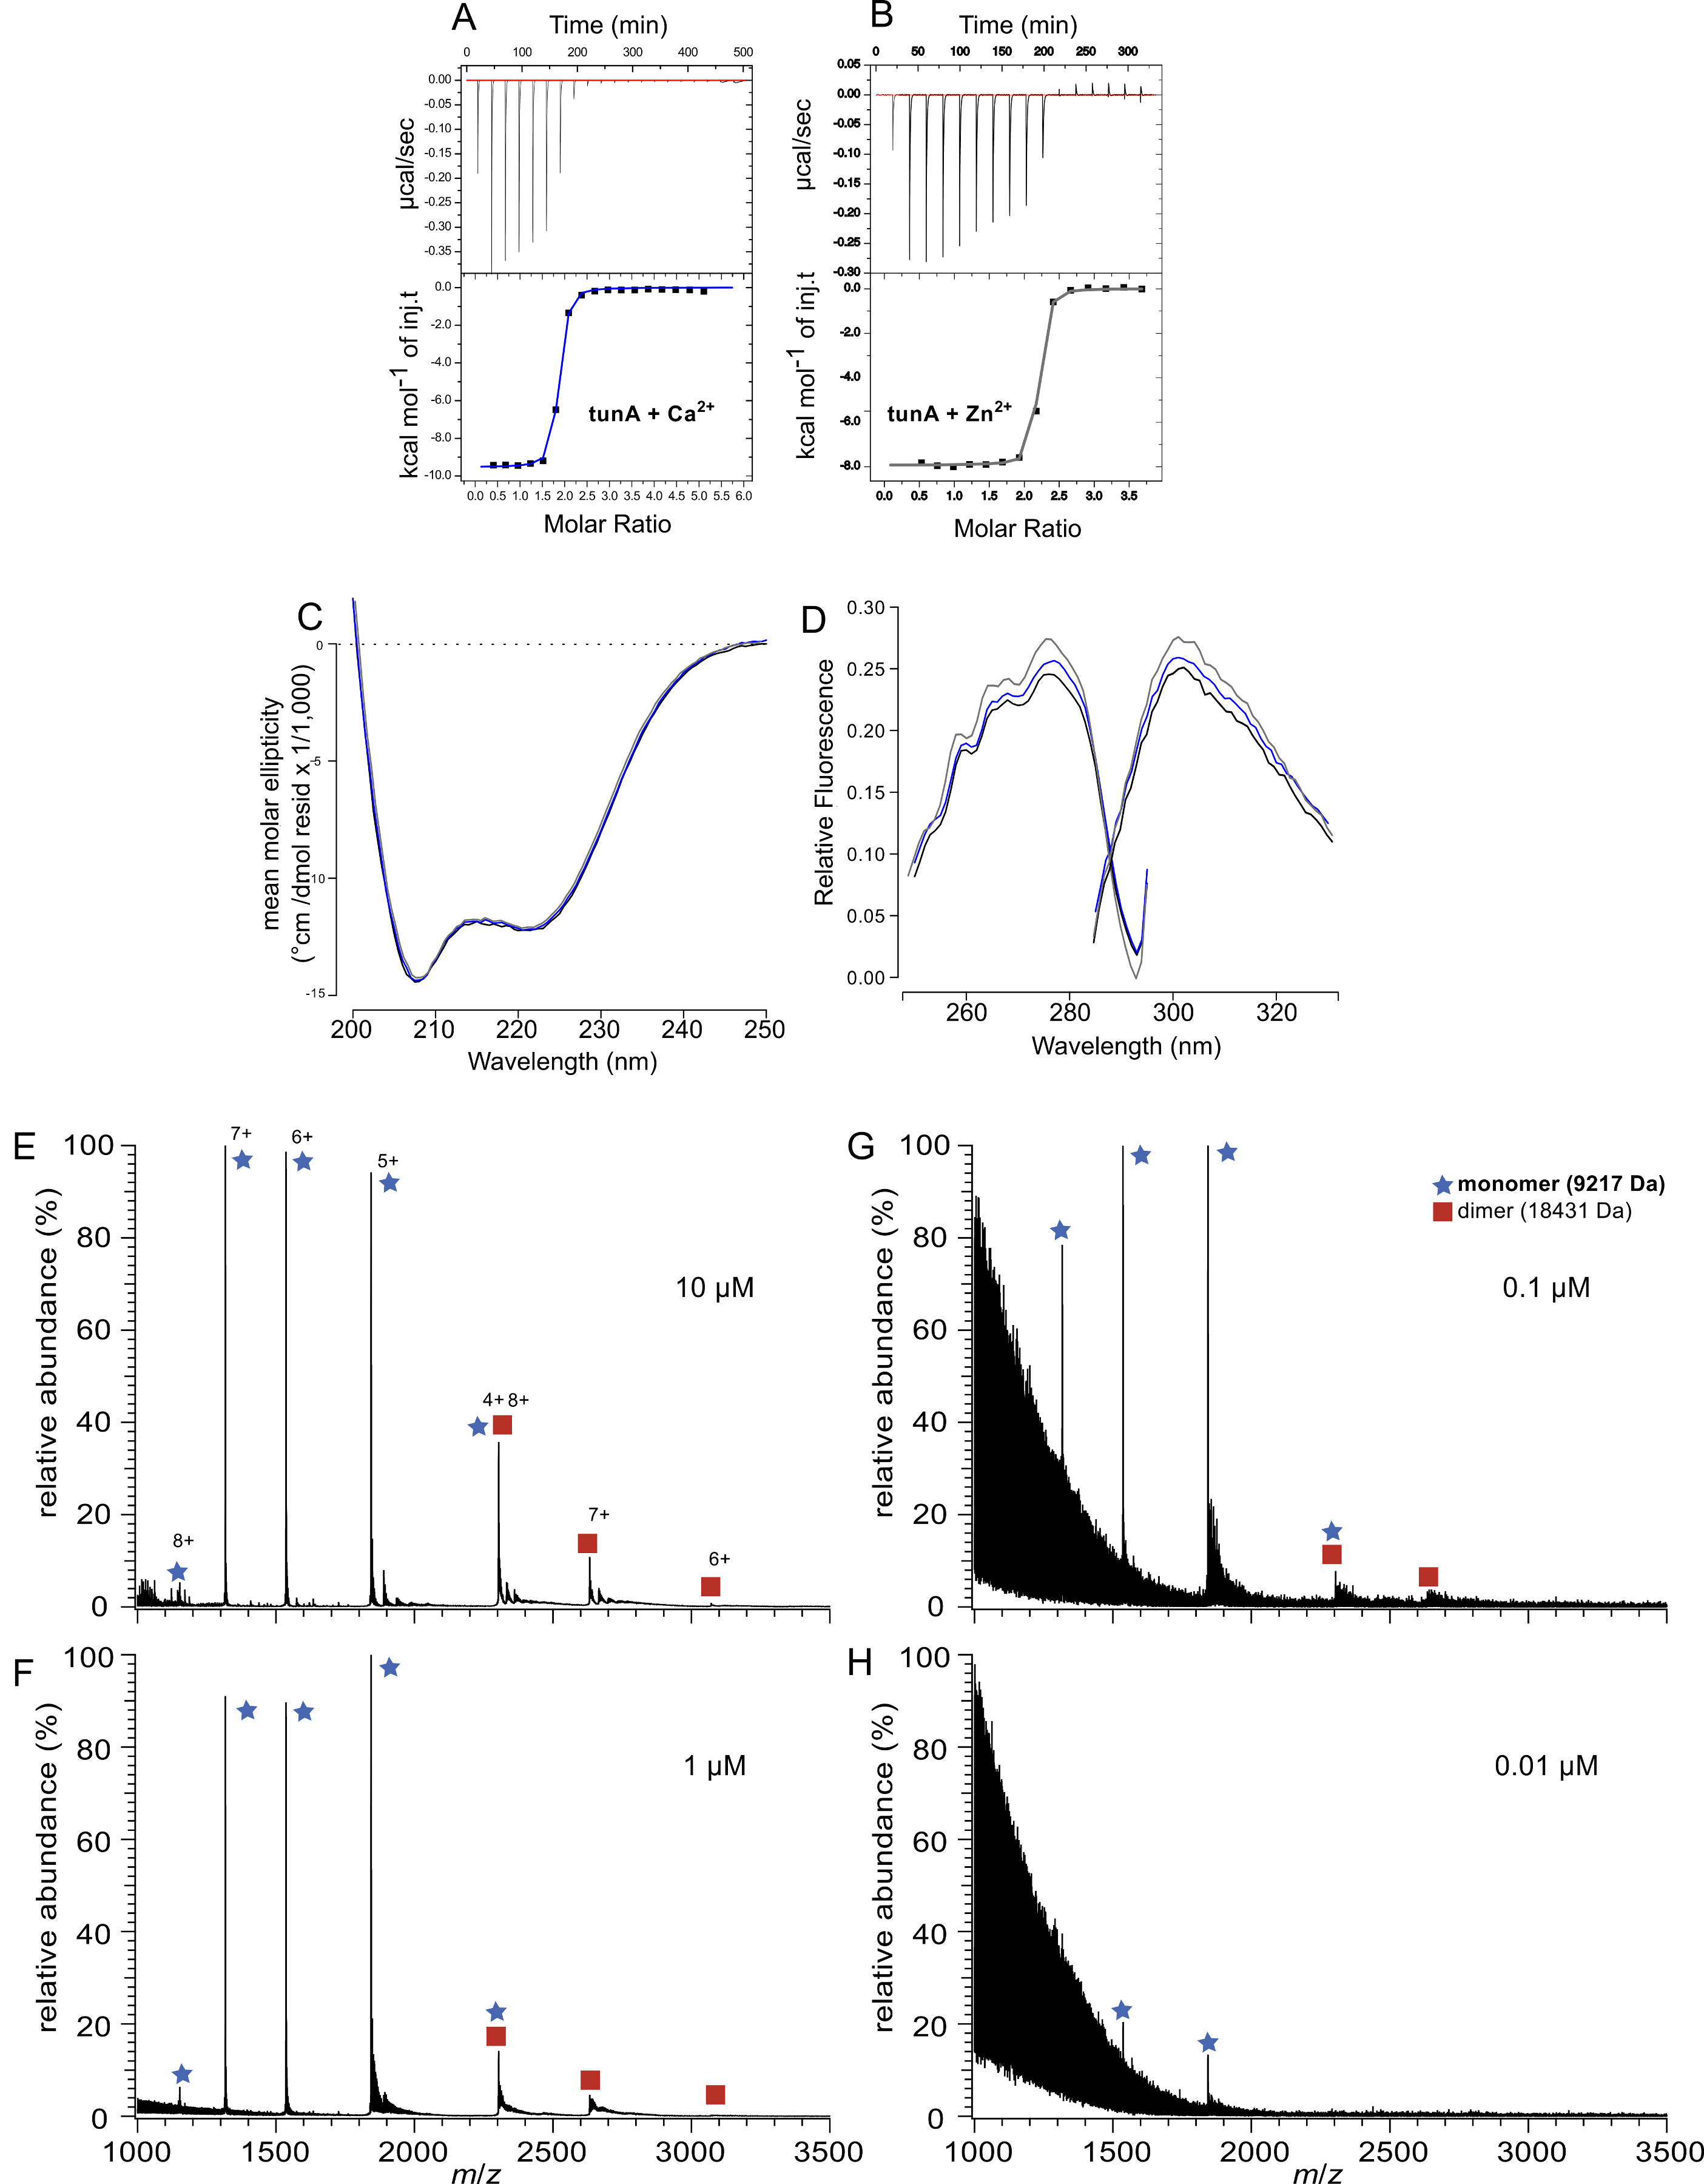
\includegraphics{ch3-S6_fig.png} 
\caption[Biophysical characterization of tunA]{A) ITC trace for binding of Ca\textsuperscript{2+}. B) ITC trace for binding of Zn\textsuperscript{2+}. C) Far-UV CD spectra for tunA in apo form (black), presence of Ca\textsuperscript{2+} (blue) and presence of Zn\textsuperscript{2+} (gray). D) Intrinsic fluorescence spectra for tunA with conditions as in panel C. E-H) ESI-MS spectra for tunA, titrating from 10 $\mu$M to 0.01 $\mu$M protein. Icons indicate species (monomer or dimer). Numbers indicate charge state. Dimer is lost preferentially during dilution, suggesting it is an artifact of electrospray process.\label{samplefigure}}	
\end{figure}


\begin{figure}
\centering
	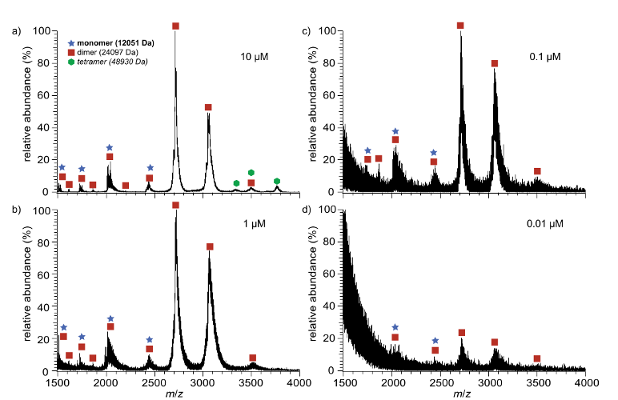
\includegraphics{ch3-S7_fig.png} 
\caption[tunB mass spectrometry dilution experiment]{tunB mass spectra at concentrations of a) 10 $\mu$M, b) 1 $\mu$M, c) 0.1 $\mu$M, and d) 0.01 $\mu$M demonstrate that tunB homodimers are robust to dilution, indicating that this is a specific interaction. Homotetramer is observed only in the most concentrated sample, thus homotetramer signal likely arises from non-specific interactions during the electrospray process.\label{samplefigure}}	
\end{figure}


\begin{figure}
\centering
	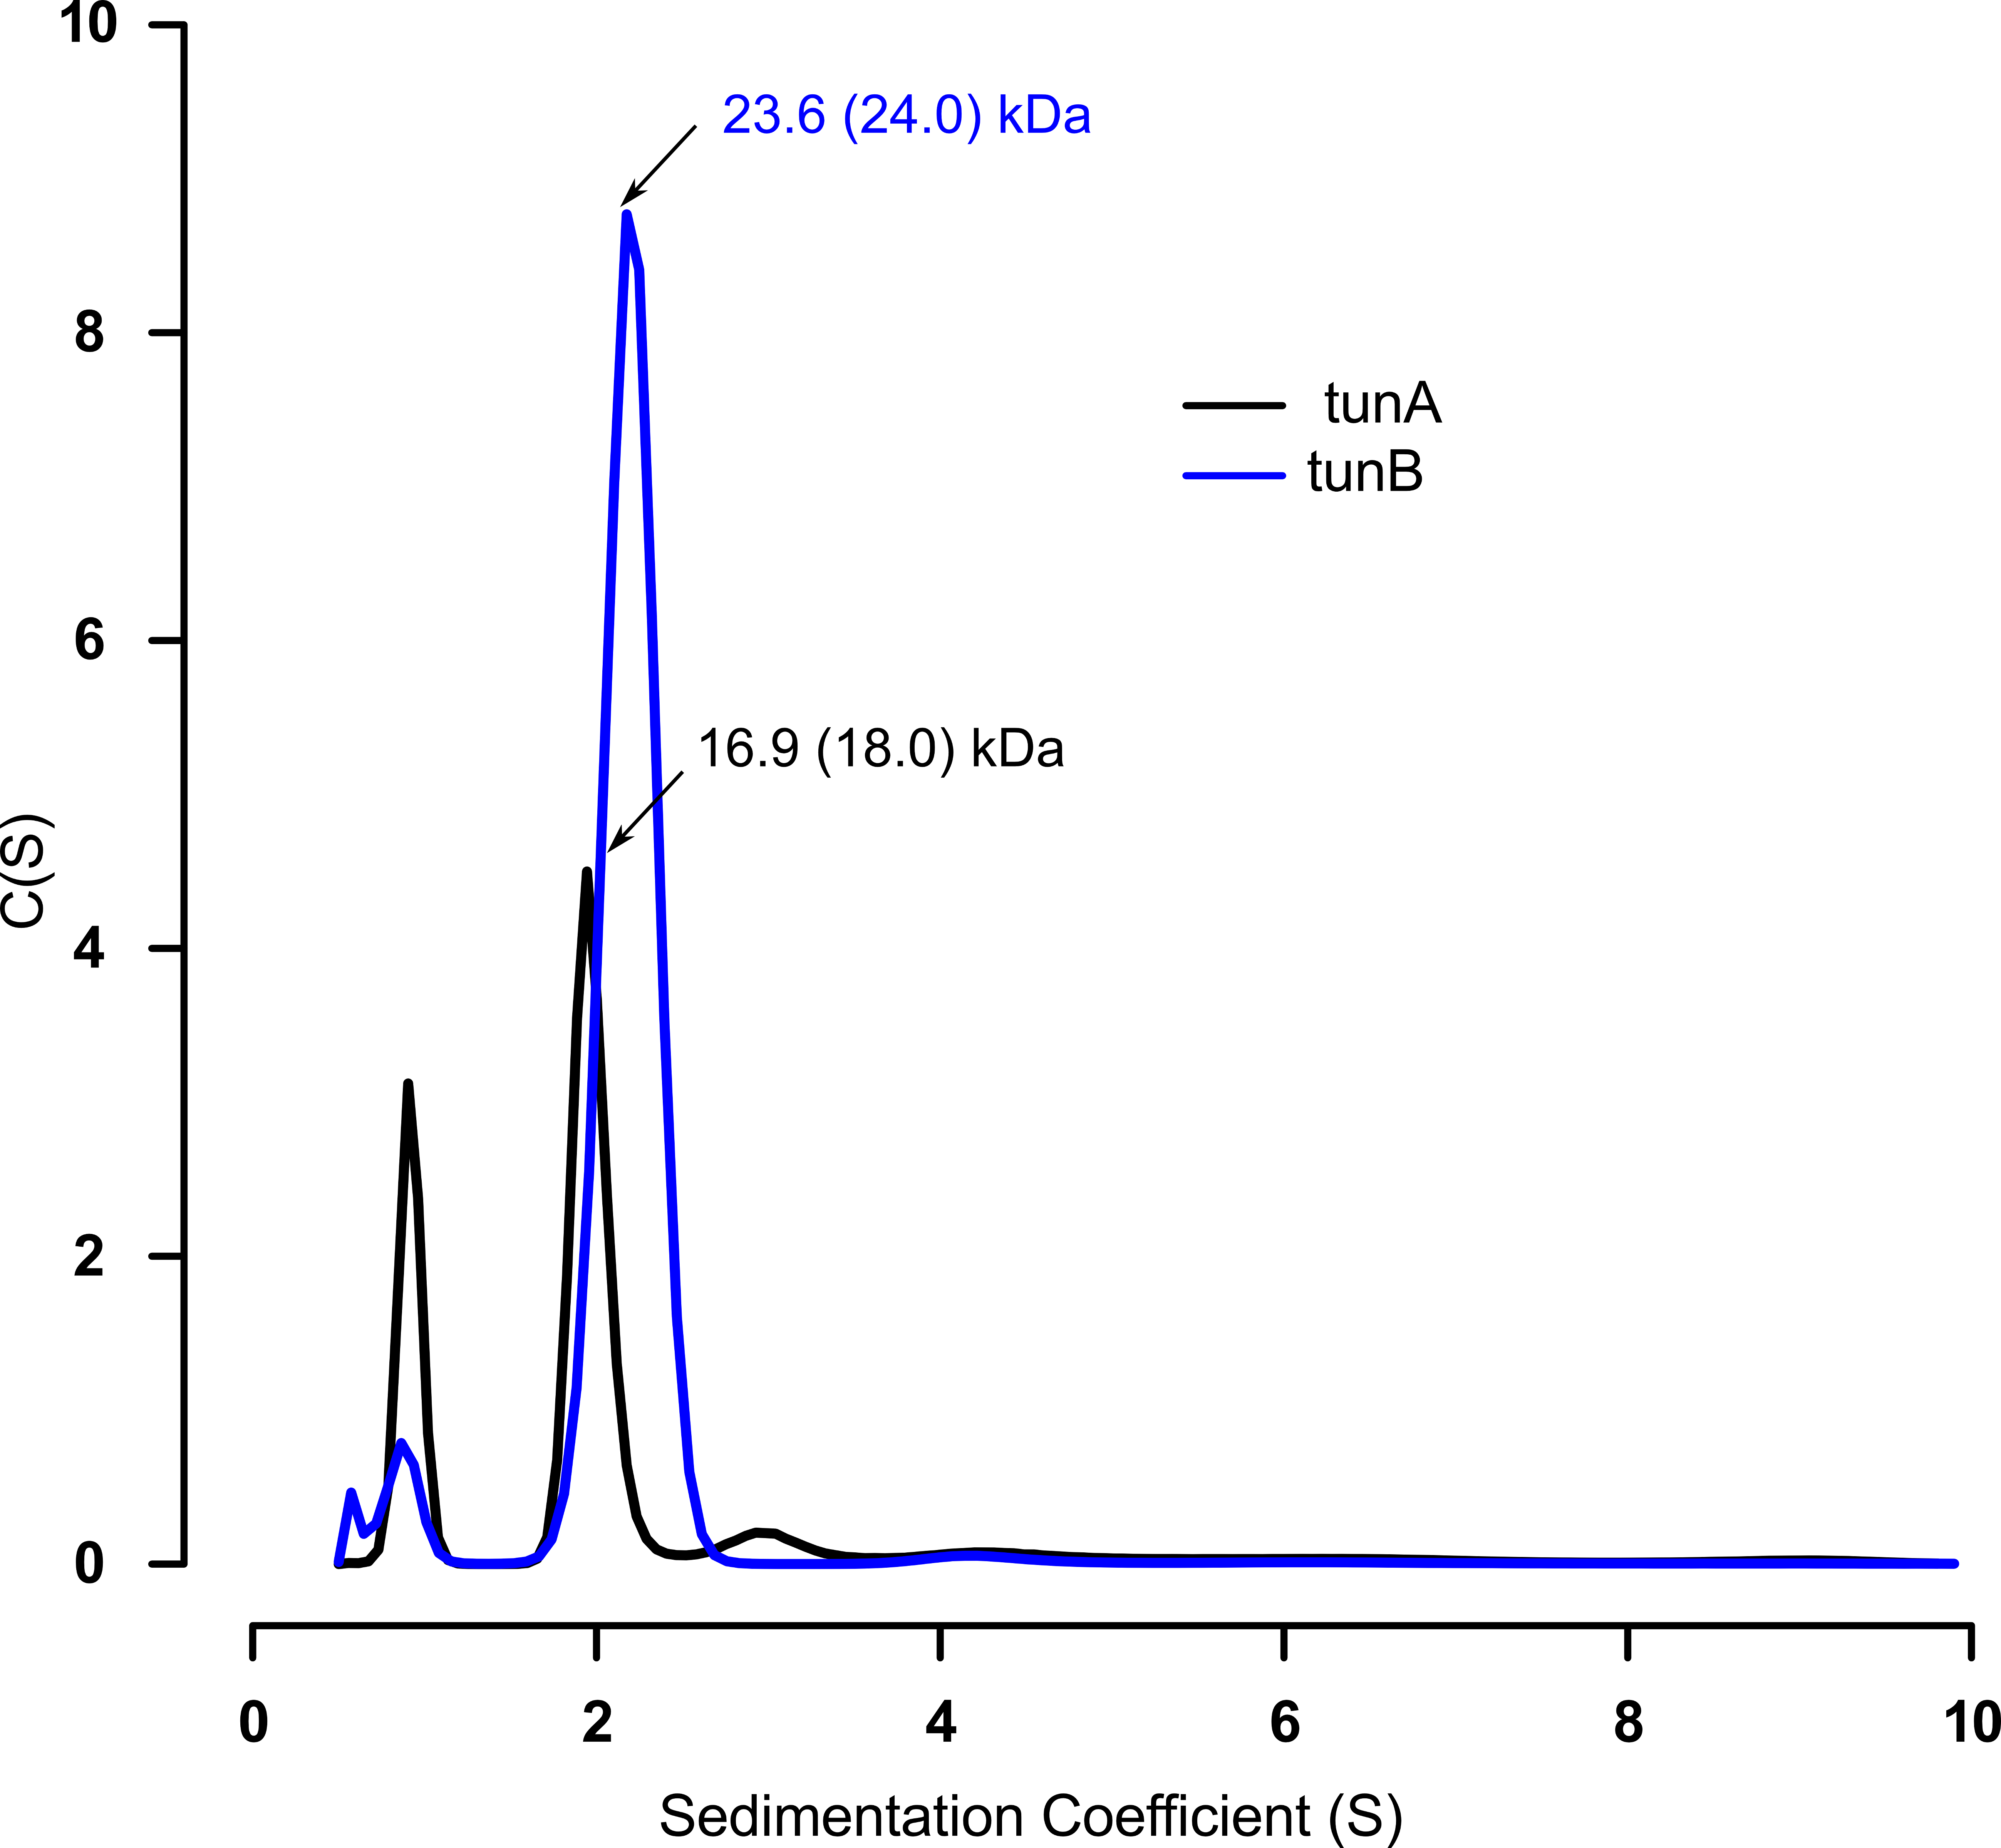
\includegraphics{ch3-S8_fig.png} 
\caption[Sedimentation velocity AUC analysis of tunA and tunB]{Graph shows the distribution of sedimentation coefficient determined for tunA (black) and tunB (blue). The apparent mass of the homodimer peaks are indicated above each peak, with the mass expected from the amino acid sequence of the protein in parentheses.\label{samplefigure}}	
\end{figure}







